\documentclass[prb,preprint]{revtex4-1} 


\usepackage{amsmath}  
\usepackage{amsfonts} 
\usepackage{graphicx} 
\usepackage{color}
\usepackage{ulem}
\begin{document}


\title{Recreating Young's Double Slit Experiment}


\author{Ed Lipchus}
\email{ejl13@hampshire.edu}
\affiliation{Department of Natural Science, Hampshire College, Amherst, MA 01002}


\author{Danika Luntz-Martin}
\email{dluntzma@smith.edu}
\affiliation{Department of Physics, Smith College, Northampton, MA 01063}


\date{\today}



\begin{abstract}


\end{abstract}

\maketitle 


\section{Introduction} 

The double slit experiment preformed by Thomas Young was seminal because it demonstrated the wave nature of light. 

\section{Methods}

We used the TeachSpin Two-Slit Interference, One Photon at a Time (TWS1-B) which is a apparatus designed to perform Young's double slit experiment. The apparatus has two light sources, a 670 nm diode laser and a light bulb with a removable green light filter. There are four slit holders spaced throughout the length of the apparatus, see Figure~\ref{apparatus}. The first slit, the source slit, is eliminates excess light from the light source and approximates a plane wave. Next is the double slit, our double slit had 0.1mm wide slits and center to center separation of 0.353mm. Following the double slit was a wide single slit attached to a micrometer, called the slit blocker. The slit blocker could be moved to block either or both slits of the double slit. Finally there was a detector slit which allowed us to measure the intensity of light (using the laser) or the number of photons (using the light bulb) over a small region of the x-axis. The micrometer attached to the detector slit allowed us to scan along the x-axis. When we worked with the laser as our light source we used the built in photodetector which gave an output voltage that was proportionate to the light intensity. When we used light bulb as our light source we used the built in photo-multiplier tube (PMT) attached to the TeachSpin Pulse Counter / Interval Timer (PCIT1) to count the number of photons.

\begin{figure}[h!]
\centering
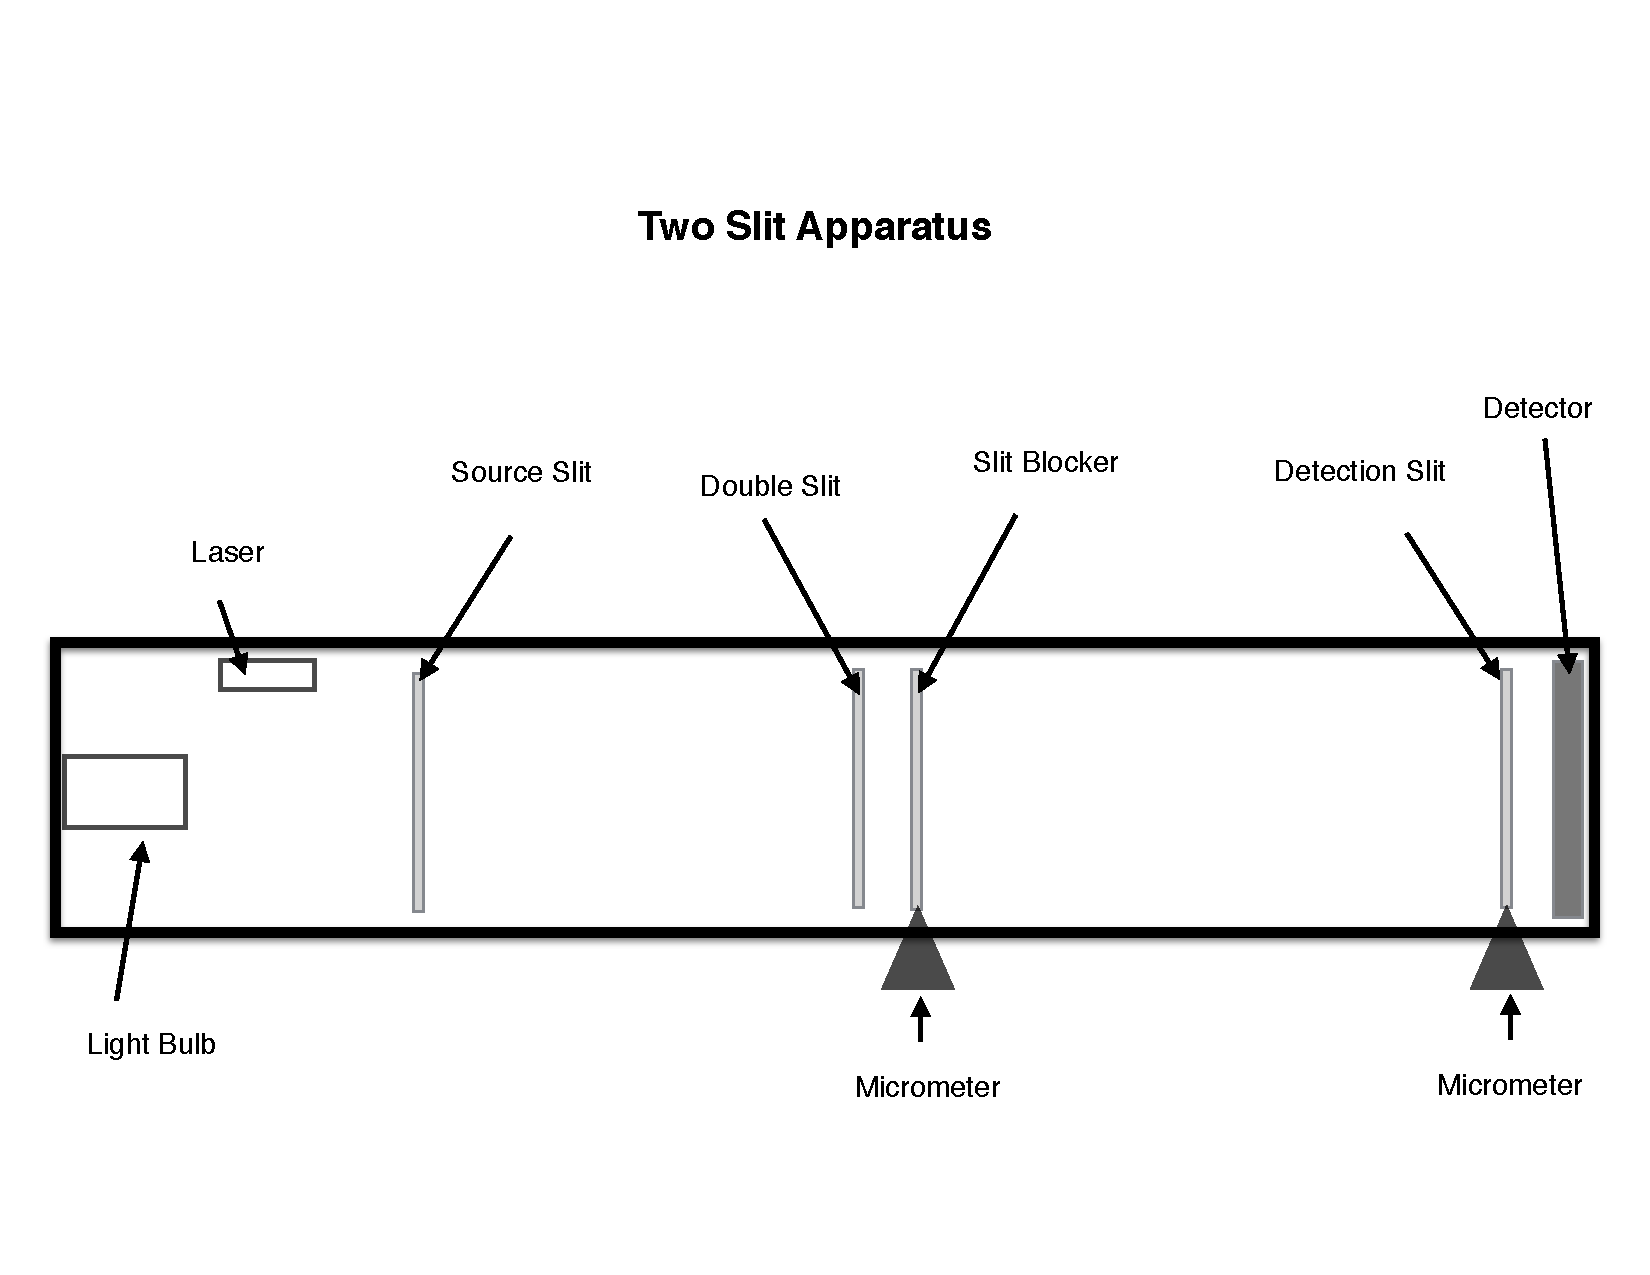
\includegraphics[width=6in]{apparatus.pdf}
\caption{The experimental set-up of the apparatus we used. The laser can slide into place in front of the light bulb. The source slit is a wide slit that blocks extraneous light from the light source. The slit blocker is another wide slit that can be moved, using the micrometer, to block one of the double slits, effectively turning it into a single slit. The detector slit allowed us to count the number of photon reaching the detector over a small region. The micrometer allowed us to scan across the detector and get a photon count at each x value.}
\label{apparatus}
\end{figure}

\section{Results}


\section{Analysis}


\section{Discussion}


\section{Conclusion}

\begin{thebibliography}{1}

\bibitem{teachspin} Jonathan F. Reichert, \textit{TeachSpin Instruction Manuals: Two-Slit Interference, One Photon at a Time (TWS1 - B), Pulse Counter / Interval Timer (PCIT1)} Rev. 1.0, (2013)

\end{thebibliography}
\end{document}
